\documentclass[12pt,a4paper]{article}
\usepackage[utf8]{inputenc}
\usepackage{amsmath}
\usepackage{amsfonts}
\usepackage{amssymb}
\usepackage{graphicx}


\usepackage{mathpazo} % Palatino font

\graphicspath{ {./images/} } % sets image folder


\begin{document}

%----------------------------------------------------------------------------------------
%	TITLE PAGE
%----------------------------------------------------------------------------------------

\begin{titlepage} % Suppresses displaying the page number on the title page and the subsequent page counts as page 1
	\newcommand{\HRule}{\rule{\linewidth}{0.5mm}} % Defines a new command for horizontal lines, change thickness here
	
	\center % Centre everything on the page
	
	%------------------------------------------------
	%	Headings
	%------------------------------------------------
	
	%\textsc{\LARGE Hochschule für Technik \& Wirtschaft Berlin}\\[1.5cm] % Main heading such as the name of your university/college
		
\includegraphics[width=0.9\textwidth]{/Users/esteban/Projects/ba-latex-code/images/logo.png}\\[1cm] % Include a department/university logo - this will require the graphicx package
	
	\textsc{\Large Bachelorarbeit}\\[0.5cm] % Major heading such as course name
	
	\textsc{\large Fachbereich 4: Internationale Medieninformatik}\\[0.5cm] % Minor heading such as course title
	
	%------------------------------------------------
	%	Title
	%------------------------------------------------
	
	\HRule\\[0.4cm]
	
	{\huge\bfseries Thunderbird Add-on: 'One Time Password/Pad' Encryption}\\[0.4cm] % Title of your document
	
	\HRule\\[1.5cm]
	
	%------------------------------------------------
	%	Author(s)
	%------------------------------------------------
	
	\begin{minipage}{0.4\textwidth}
		\begin{flushleft}
			\large
			\textit{Student}\\
			Esteban \textsc{Licea} % Your name
		\end{flushleft}
	\end{minipage}
	~
	\begin{minipage}{0.4\textwidth}
		\begin{flushright}
			\large
			\textit{Mentor/Supervisor}\\
			Prof. Dr. Debora \textsc{Weber-Wulff} % Supervisor's name
		\end{flushright}
	\end{minipage}
	
	% If you don't want a supervisor, uncomment the two lines below and comment the code above
	%{\large\textit{Author}}\\
	%John \textsc{Smith} % Your name
	
	%------------------------------------------------
	%	Date
	%------------------------------------------------
	
	\vfill\vfill\vfill % Position the date 3/4 down the remaining page
	
	{\large\today} % Date, change the \today to a set date if you want to be precise
	
	%------------------------------------------------
	%	Logo
	%------------------------------------------------
	
	%\vfill\vfill

	 
	%----------------------------------------------------------------------------------------
	
	\vfill % Push the date up 1/4 of the remaining page
	
\end{titlepage}

\tableofcontents
\newpage

\section{Specifications details}

% This tex file holds the personas png images made with another
% external website/program
\newpage
\subsection{Personas}

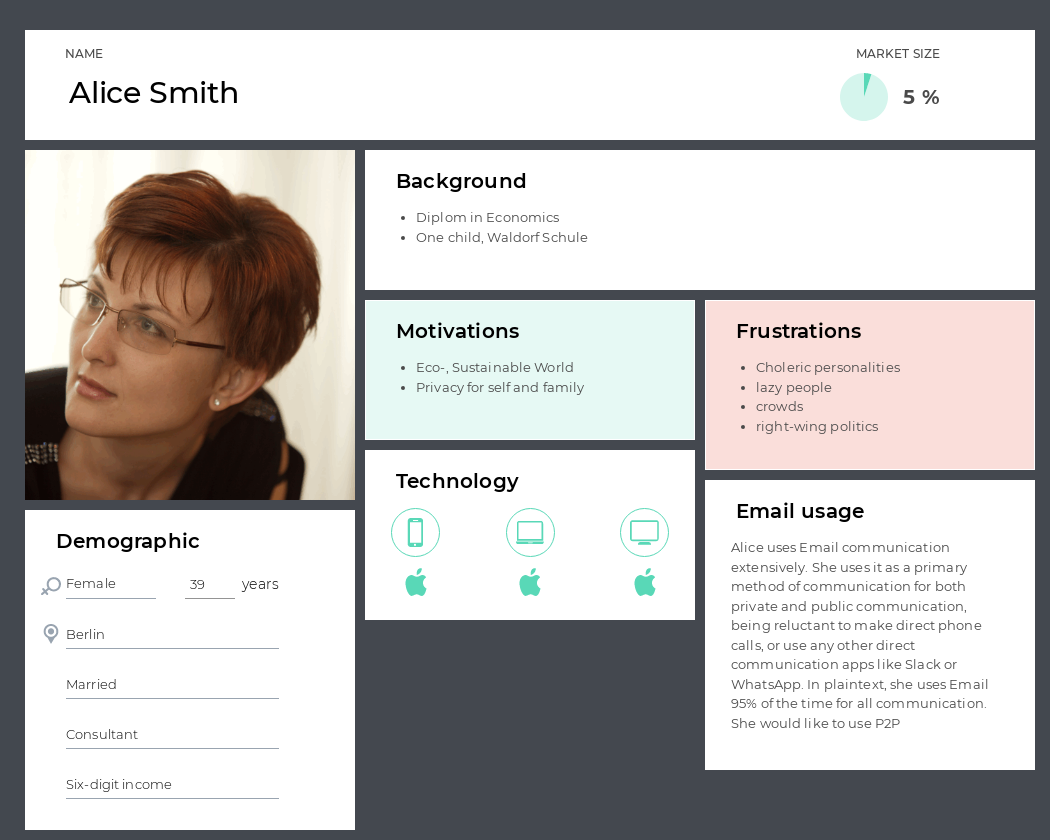
\includegraphics[scale=.38]{Alice Smith.png}
\\
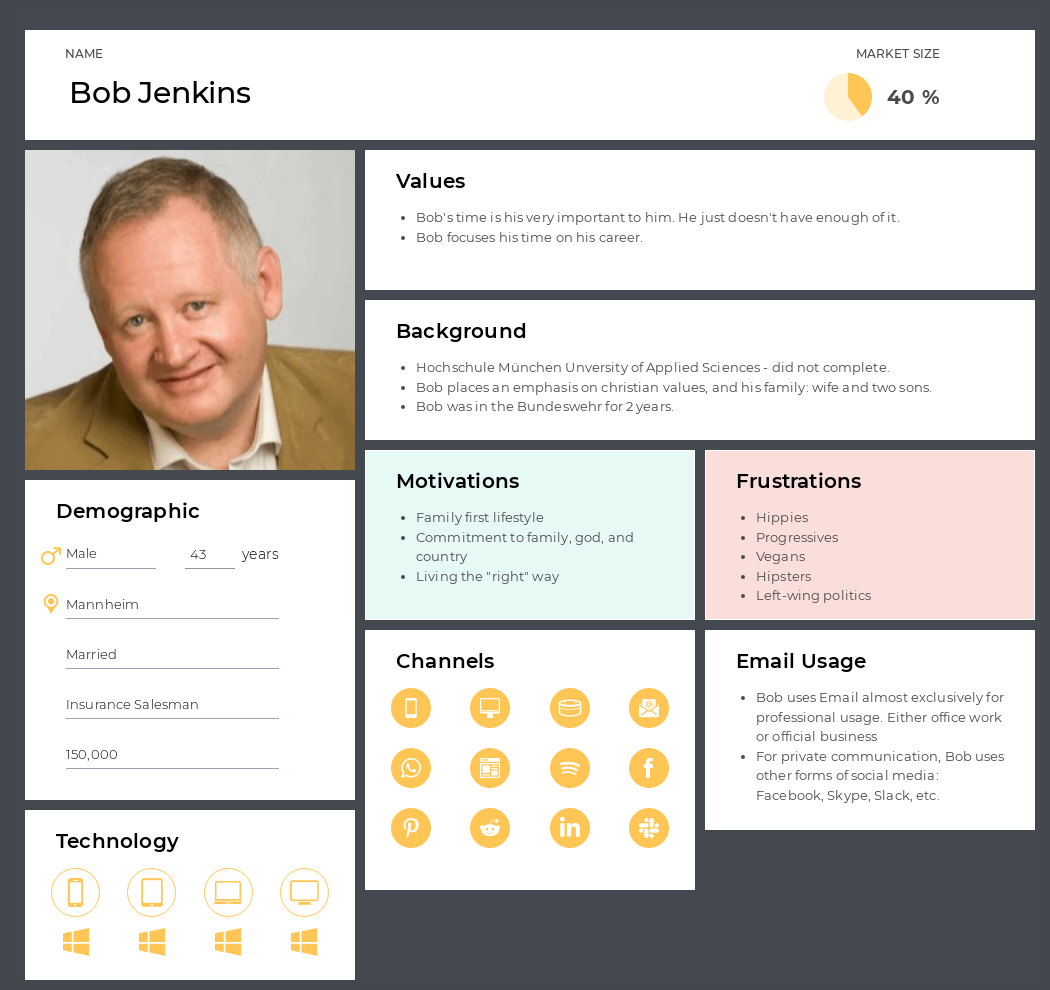
\includegraphics[scale=.38]{Bob Jenkins.png}

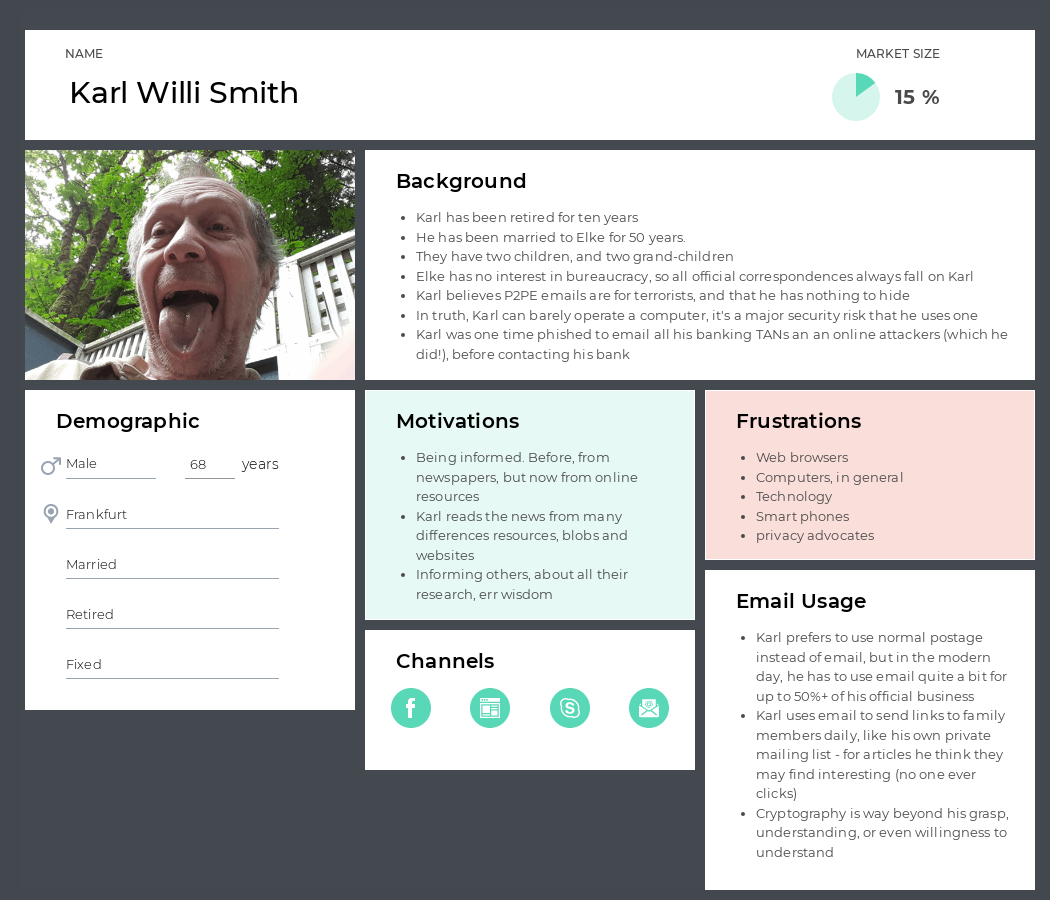
\includegraphics[scale=.38]{Karl Willi Smith.png}

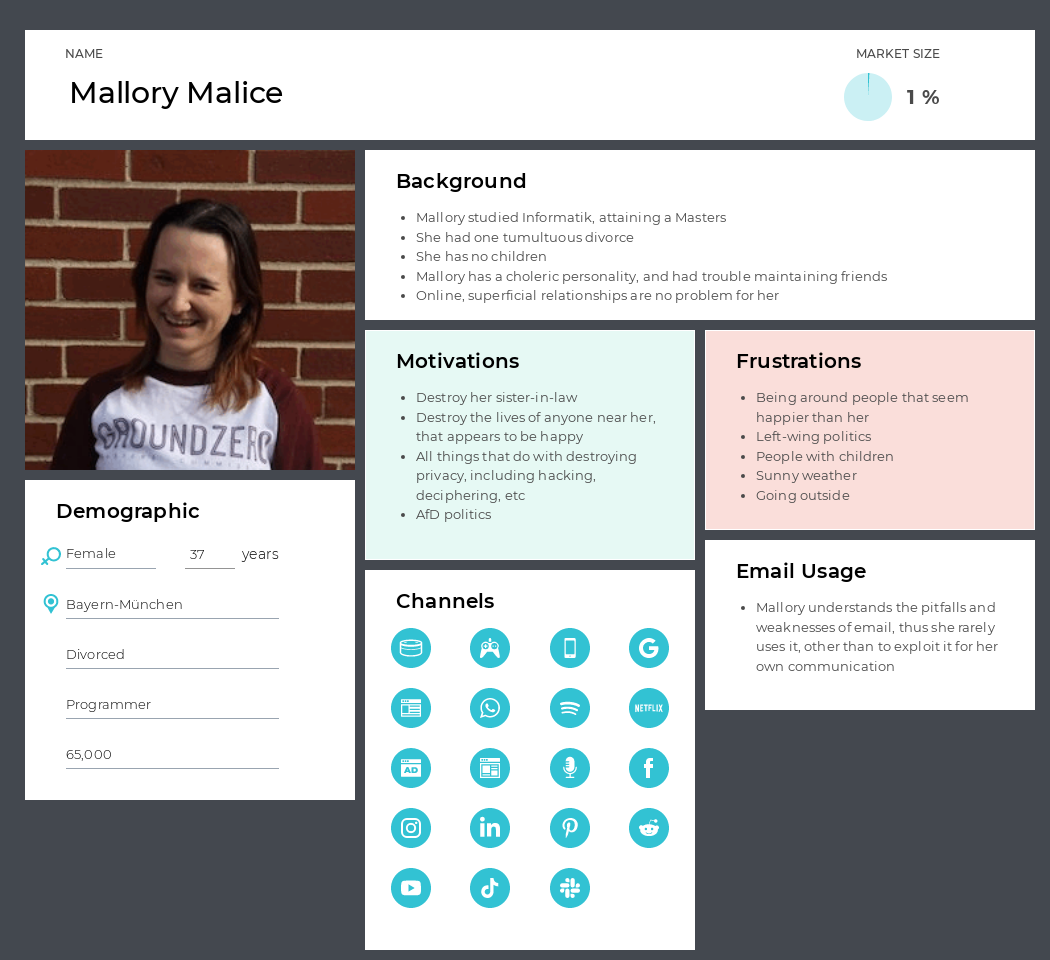
\includegraphics[scale=.38]{Mallory Malice.png}





%The following section will contain the 
\subsection{Use Cases}
\paragraph{The Use Cases used in this project will be defined, and or be restricted to the following items:}
\subsubsection{Use Case ID}
\paragraph{The Use Case ID will be a unique, numeric identifier for the use case.}

\subsubsection{Actor(s)}
\paragraph{An actor is a person or other entity external to the system who interacts with it, and performs use cases to complete task. Included in this designation, will be additional actors who participate in the use case.}

\subsubsection{Description}
\paragraph{This section should describe at a high level the purpose of the use case, what it aims to achieve, and any other relevant outcomes.}

\subsubsection{Preconditions}
\paragraph{The preconditions are all those conditions that must exist prior to the execution of the use case.}

\subsubsection{Basic Flow}
\paragraph{These are the basic, ordered steps and the description required for the completion of the use case. The steps will be numbers, and should be executed in this exact order. Completing the steps, in this order, should lead to the completion of the use case without error.}

\subsubsection{Exceptions}
\paragraph{Describes any anticipated errors that could occur during the execution of the use case, and how the system will handle these errors. The exceptions systems will not describe unanticipated errors, or error that are not included in the basic flow.}

\subsubsection{Postconditions}
\paragraph{Describes the state of all relevant parties, including the system, \emph{after} the execution of the use case.}
\newpage


\begin{longtable} {|p{3cm}|p{9cm}|} %[!htb]
%\begin{center}
%\resizebox {12cm}{!}{
%	\begin{tabular}{|p{2cm}|p{10cm}|}
	\hline
	%added the multicolumn command here to be able to make titles across different columns.
	%\multicolumn{2}{|c|}{Use Cases}\\ 
	%\hline
Use Case ID: & 0\\
	\hline
Actor(s): & Alice \\
	\hline
Description: & Alice will encrypt an email to Bob \\
	\hline
	\multicolumn{2}{|l|}{Preconditions:} \\
	\multicolumn{2}{|l|}{1. Thunderbird Email client installed.} \\
	\multicolumn{2}{|l|}{2. Thunderbird Email client configured to send and receive emails.}\\
	\multicolumn{2}{|l|}{3. Super-duper Addon installed.} \\
	\multicolumn{2}{|l|}{4. Email written} \\
	\hline
	\multicolumn{2}{|l|}{Basic Flow:} \\
	\multicolumn{2}{|l|}{1. Alice writes an email in Thunderbird.}\\
	\multicolumn{2}{|l|}{2. Alice locates and click on the add-on button.} \\
	\multicolumn{2}{|l|}{3. Observe: Alive sees a popup screen encrypt the email.} \\
	\multicolumn{2}{|l|}{4. Alice is prompted to enter a password.}\\
	\hline
	\hline
	\multicolumn{2}{|l|}{Exceptions:} \\
	\multicolumn{2}{|l|}{1. N/A} \\
%	\multicolumn{2}{|l|}{2.} \\
%	\multicolumn{2}{|l|}{3.} \\
%	\multicolumn{2}{|l|}{4.} \\
	\hline
	\hline
	\multicolumn{2}{|l|}{Postconditions:} \\
	\multicolumn{2}{|l|}{1. The email is enciphered.} \\
	\multicolumn{2}{|l|}{2. The addon window closes.} \\
	\multicolumn{2}{|l|}{3. Alice is returned to the Thunderbird client.} \\
	%\multicolumn{2}{|l|}{4.} \\
	\hline
\end{longtable}

%\begin{longtable} {|p{3cm}|p{9cm}|} %[!htb]
%%\begin{center}
%%\resizebox {12cm}{!}{
%%	\begin{tabular}{|p{2cm}|p{10cm}|}
%	\hline
%	%added the multicolumn command here to be able to make titles across different columns.
%	%\multicolumn{2}{|c|}{Use Cases}\\ 
%	%\hline
%Use Case ID: & 001\\
%	\hline
%Actor(s): & Alice Smith \\
%	\hline
%Description: & Alice cancels the processing of an email. \\
%	\hline
%	\multicolumn{2}{|l|}{Preconditions:} \\
%	\multicolumn{2}{|l|}{1. Thunderbird Email client installed.} \\
%	\multicolumn{2}{|l|}{2. Thunderbird Email client configured to send and receive emails.}\\
%	\multicolumn{2}{|l|}{3. Super-duper Add-on installed.} \\
%	\multicolumn{2}{|l|}{4. Email written} \\
%	\hline
%	\multicolumn{2}{|l|}{Basic Flow:} \\
%	\multicolumn{2}{|l|}{1. Alice writes an email in Thunderbird.}\\
%	\multicolumn{2}{|l|}{2. Alice locates and click on the Add-on button.} \\
%	\multicolumn{2}{|l|}{3. Observe: Alive sees a popup screen encrypt the email.} \\
%	\multicolumn{2}{|l|}{4. Alice is prompted to enter a password.}\\
%	\hline
%	\hline
%	\multicolumn{2}{|l|}{Exceptions:} \\
%	\multicolumn{2}{|l|}{1. Between every number option above, Alice can cancel the email.} \\
%%	\multicolumn{2}{|l|}{2.} \\
%%	\multicolumn{2}{|l|}{3.} \\
%%	\multicolumn{2}{|l|}{4.} \\
%	\hline
%	\hline
%	\multicolumn{2}{|l|}{Postconditions:} \\
%	\multicolumn{2}{|l|}{1. The email encryption is canceled.} \\
%	\multicolumn{2}{|l|}{2. The Add-on window closes.} \\
%	\multicolumn{2}{|l|}{3. Alice is returned to the Thunderbird client.} \\
%	%\multicolumn{2}{|l|}{4.} \\
%	\hline
%\end{longtable}

\begin{longtable} {|p{3cm}|p{9cm}|} %[!htb]
%\begin{center}
%\resizebox {12cm}{!}{
%	\begin{tabular}{|p{2cm}|p{10cm}|}
	\hline
	%added the multicolumn command here to be able to make titles across different columns.
	%\multicolumn{2}{|c|}{Use Cases}\\ 
	%\hline
Use Case ID: & 1\\
	\hline
Actor(s): & Bob (or any other intended recipient) decrypts an Email from Alice \\
	\hline
Description: & Alice will encrypt an email to another actor, then share a password with them, that they will then be able to decrypt \\
	\hline
	\multicolumn{2}{|l|}{Preconditions:} \\
	\multicolumn{2}{|l|}{1. Thunderbird Email client installed.} \\
	\multicolumn{2}{|l|}{2. Thunderbird Email client configured to send and receive emails.}\\
	\multicolumn{2}{|l|}{3. Super-duper Add-on installed.} \\
	\multicolumn{2}{|l|}{4. Email written} \\
	\hline
	\multicolumn{2}{|l|}{Basic Flow:} \\
	\multicolumn{2}{|l|}{1. Alice writes an email in Thunderbird.}\\
	\multicolumn{2}{|l|}{2. Alice locates and click on the addon button.} \\
	\multicolumn{2}{|l|}{3. Observe: Alive sees a popup screen encrypt the email.} \\
	\multicolumn{2}{|l|}{4. Alice is prompted to enter a password.}\\
	\multicolumn{2}{|l|}{5. Alice enters a password.} \\
	\multicolumn{2}{|l|}{4. Alice shares this password with said actor \emph{offline}.}\\
	\hline
	\hline
	\multicolumn{2}{|l|}{Exceptions:} \\
	\multicolumn{2}{|l|}{1. N/A} \\
%	\multicolumn{2}{|l|}{2.} \\
%	\multicolumn{2}{|l|}{3.} \\
%	\multicolumn{2}{|l|}{4.} \\
	\hline
	\hline
	\multicolumn{2}{|l|}{Postconditions:} \\
	\multicolumn{2}{|l|}{1. The email is enciphered.} \\
	\multicolumn{2}{|l|}{2. The addon window closes.} \\
	\multicolumn{2}{|l|}{3. Alice is returned to the Thunderbird client.} \\
	%\multicolumn{2}{|l|}{4.} \\
	\hline
\end{longtable}

%
%\begin{longtable} {|p{3cm}|p{9cm}|} %[!htb]
%%\begin{center}
%%\resizebox {12cm}{!}{
%%	\begin{tabular}{|p{2cm}|p{10cm}|}
%	\hline
%	%added the multicolumn command here to be able to make titles across different columns.
%	%\multicolumn{2}{|c|}{Use Cases}\\ 
%	%\hline
%Use Case ID: & 2\\
%	\hline
%Actor(s): & Bob (or any other intended recipient)\\
%	\hline
%Description: & Bob will decipher an email sent from Alice.\\
%	\hline
%	\multicolumn{2}{|l|}{Preconditions:} \\
%	\multicolumn{2}{|l|}{1. Thunderbird Email client installed.} \\
%	\multicolumn{2}{|l|}{2. Thunderbird Email client configured to send and receive emails.}\\
%	\multicolumn{2}{|l|}{3. Super-duper Add-on installed.} \\
%	\multicolumn{2}{|l|}{4. Enciphered Email received.} \\
%	\multicolumn{2}{|l|}{5. Deciphering password from Alice Smith received.} \\
%	\hline
%	\multicolumn{2}{|l|}{Basic Flow:} \\
%	\multicolumn{2}{|l|}{1. Bob opens his Thunderbird email client.}\\
%	\multicolumn{2}{|l|}{2. Bob notices an encrypted email from Alice in his inbox.} \\
%	\multicolumn{2}{|l|}{3. Bob selects the email.} \\
%	\multicolumn{2}{|l|}{3. Observe: A popup window appears, prompting Bob for a password.} \\
%	\multicolumn{2}{|l|}{4. Bob enters the password.}\\
%	\multicolumn{2}{|l|}{3. The email is deciphered, and can now be read.} \\
%	\hline
%	\hline
%	\multicolumn{2}{|l|}{Exceptions:} \\
%	\multicolumn{2}{|l|}{1. N/A} \\
%%	\multicolumn{2}{|l|}{2.} \\
%%	\multicolumn{2}{|l|}{3.} \\
%%	\multicolumn{2}{|l|}{4.} \\
%	\hline
%	\hline
%	\multicolumn{2}{|l|}{Postconditions:} \\
%	\multicolumn{2}{|l|}{1. The prompting window disappears.} \\
%	\multicolumn{2}{|l|}{2. The email can now be read..} \\
%%	\multicolumn{2}{|l|}{3. Alice is returned to the Thunderbird client.} \\
%	%\multicolumn{2}{|l|}{4.} \\
%	\hline
%\end{longtable}


%\begin{longtable} {|p{3cm}|p{9cm}|} %[!htb]
%\begin{center}
%\resizebox {12cm}{!}{
%	\begin{tabular}{|p{2cm}|p{10cm}|}
	%\hline
	%added the multicolumn command here to be able to make titles across different columns.
	%\multicolumn{2}{|c|}{Use Cases}\\ 
	%\hline
%Use Case ID: & 004\\
%	\hline
%Actor(s): & Alice Smith \\
%	\hline
%Description: & Alice will encrypt an email to Bob \\
%	\hline
%	\multicolumn{2}{|l|}{Preconditions:} \\
%	\multicolumn{2}{|l|}{1. Thunderbird Email client installed.} \\
%	\multicolumn{2}{|l|}{2. Thunderbird Email client configured to send and receive emails.}\\
%	\multicolumn{2}{|l|}{3. Super-duper Addon installed.} \\
%	\multicolumn{2}{|l|}{4. Email written} \\
%	\hline
%	\multicolumn{2}{|l|}{Basic Flow:} \\
%	\multicolumn{2}{|l|}{1. Alice writes an email in Thunderbird.}\\
%	\multicolumn{2}{|l|}{2. Alice locates and click on the addon button.} \\
%	\multicolumn{2}{|l|}{3. Observe: Alive sees a popup screen encrypt the email.} \\
%	\multicolumn{2}{|l|}{4. Alice is prompted to enter a password.}\\
%	\hline
%	\hline
%	\multicolumn{2}{|l|}{Exceptions:} \\
%	\multicolumn{2}{|l|}{1. None allowed. =)} \\
%%	\multicolumn{2}{|l|}{2.} \\
%%	\multicolumn{2}{|l|}{3.} \\
%%	\multicolumn{2}{|l|}{4.} \\
%	\hline
%	\hline
%	\multicolumn{2}{|l|}{Postconditions:} \\
%	\multicolumn{2}{|l|}{1. The email is enciphered.} \\
%	\multicolumn{2}{|l|}{2. The addon window closes.} \\
%	\multicolumn{2}{|l|}{3. Alice is returned to the Thunderbird client.} \\
%	%\multicolumn{2}{|l|}{4.} \\
%	\hline
%\end{longtable}
%
%
%\begin{longtable} {|p{3cm}|p{9cm}|} %[!htb]
%%\begin{center}
%%\resizebox {12cm}{!}{
%%	\begin{tabular}{|p{2cm}|p{10cm}|}
%	\hline
%	%added the multicolumn command here to be able to make titles across different columns.
%	%\multicolumn{2}{|c|}{Use Cases}\\ 
%	%\hline
%Use Case ID: & 005\\
%	\hline
%Actor(s): & Alice Smith \\
%	\hline
%Description: & Alice will encrypt an email to Bob \\
%	\hline
%	\multicolumn{2}{|l|}{Preconditions:} \\
%	\multicolumn{2}{|l|}{1. Thunderbird Email client installed.} \\
%	\multicolumn{2}{|l|}{2. Thunderbird Email client configured to send and receive emails.}\\
%	\multicolumn{2}{|l|}{3. Super-duper Addon installed.} \\
%	\multicolumn{2}{|l|}{4. Email written} \\
%	\hline
%	\multicolumn{2}{|l|}{Basic Flow:} \\
%	\multicolumn{2}{|l|}{1. Alice writes an email in Thunderbird.}\\
%	\multicolumn{2}{|l|}{2. Alice locates and click on the addon button.} \\
%	\multicolumn{2}{|l|}{3. Observe: Alive sees a popup screen encrypt the email.} \\
%	\multicolumn{2}{|l|}{4. Alice is prompted to enter a password.}\\
%	\hline
%	\hline
%	\multicolumn{2}{|l|}{Exceptions:} \\
%	\multicolumn{2}{|l|}{1. None allowed. =)} \\
%%	\multicolumn{2}{|l|}{2.} \\
%%	\multicolumn{2}{|l|}{3.} \\
%%	\multicolumn{2}{|l|}{4.} \\
%	\hline
%	\hline
%	\multicolumn{2}{|l|}{Postconditions:} \\
%	\multicolumn{2}{|l|}{1. The email is enciphered.} \\
%	\multicolumn{2}{|l|}{2. The addon window closes.} \\
%	\multicolumn{2}{|l|}{3. Alice is returned to the Thunderbird client.} \\
%	%\multicolumn{2}{|l|}{4.} \\
%	\hline
%\end{longtable}
%
%
%\begin{longtable} {|p{3cm}|p{9cm}|} %[!htb]
%%\begin{center}
%%\resizebox {12cm}{!}{
%%	\begin{tabular}{|p{2cm}|p{10cm}|}
%	\hline
%	%added the multicolumn command here to be able to make titles across different columns.
%	%\multicolumn{2}{|c|}{Use Cases}\\ 
%	%\hline
%Use Case ID: & 006\\
%	\hline
%Actor(s): & Alice Smith \\
%	\hline
%Description: & Alice will encrypt an email to Bob \\
%	\hline
%	\multicolumn{2}{|l|}{Preconditions:} \\
%	\multicolumn{2}{|l|}{1. Thunderbird Email client installed.} \\
%	\multicolumn{2}{|l|}{2. Thunderbird Email client configured to send and receive emails.}\\
%	\multicolumn{2}{|l|}{3. Super-duper Addon installed.} \\
%	\multicolumn{2}{|l|}{4. Email written} \\
%	\hline
%	\multicolumn{2}{|l|}{Basic Flow:} \\
%	\multicolumn{2}{|l|}{1. Alice writes an email in Thunderbird.}\\
%	\multicolumn{2}{|l|}{2. Alice locates and click on the addon button.} \\
%	\multicolumn{2}{|l|}{3. Observe: Alive sees a popup screen encrypt the email.} \\
%	\multicolumn{2}{|l|}{4. Alice is prompted to enter a password.}\\
%	\hline
%	\hline
%	\multicolumn{2}{|l|}{Exceptions:} \\
%	\multicolumn{2}{|l|}{1. None allowed. =)} \\
%%	\multicolumn{2}{|l|}{2.} \\
%%	\multicolumn{2}{|l|}{3.} \\
%%	\multicolumn{2}{|l|}{4.} \\
%	\hline
%	\hline
%	\multicolumn{2}{|l|}{Postconditions:} \\
%	\multicolumn{2}{|l|}{1. The email is enciphered.} \\
%	\multicolumn{2}{|l|}{2. The addon window closes.} \\
%	\multicolumn{2}{|l|}{3. Alice is returned to the Thunderbird client.} \\
%	%\multicolumn{2}{|l|}{4.} \\
%	\hline
%\end{longtable}
%
%
%\begin{longtable} {|p{3cm}|p{9cm}|} %[!htb]
%%\begin{center}
%%\resizebox {12cm}{!}{
%%	\begin{tabular}{|p{2cm}|p{10cm}|}
%	\hline
%	%added the multicolumn command here to be able to make titles across different columns.
%	%\multicolumn{2}{|c|}{Use Cases}\\ 
%	%\hline
%Use Case ID: & 007\\
%	\hline
%Actor(s): & Alice Smith \\
%	\hline
%Description: & Alice will encrypt an email to Bob \\
%	\hline
%	\multicolumn{2}{|l|}{Preconditions:} \\
%	\multicolumn{2}{|l|}{1. Thunderbird Email client installed.} \\
%	\multicolumn{2}{|l|}{2. Thunderbird Email client configured to send and receive emails.}\\
%	\multicolumn{2}{|l|}{3. Super-duper Addon installed.} \\
%	\multicolumn{2}{|l|}{4. Email written} \\
%	\hline
%	\multicolumn{2}{|l|}{Basic Flow:} \\
%	\multicolumn{2}{|l|}{1. Alice writes an email in Thunderbird.}\\
%	\multicolumn{2}{|l|}{2. Alice locates and click on the addon button.} \\
%	\multicolumn{2}{|l|}{3. Observe: Alive sees a popup screen encrypt the email.} \\
%	\multicolumn{2}{|l|}{4. Alice is prompted to enter a password.}\\
%	\hline
%	\hline
%	\multicolumn{2}{|l|}{Exceptions:} \\
%	\multicolumn{2}{|l|}{1. None allowed. =)} \\
%%	\multicolumn{2}{|l|}{2.} \\
%%	\multicolumn{2}{|l|}{3.} \\
%%	\multicolumn{2}{|l|}{4.} \\
%	\hline
%	\hline
%	\multicolumn{2}{|l|}{Postconditions:} \\
%	\multicolumn{2}{|l|}{1. The email is enciphered.} \\
%	\multicolumn{2}{|l|}{2. The addon window closes.} \\
%	\multicolumn{2}{|l|}{3. Alice is returned to the Thunderbird client.} \\
%	%\multicolumn{2}{|l|}{4.} \\
%	\hline
%\end{longtable}
%
%\begin{longtable} {|p{3cm}|p{9cm}|} %[!htb]
%%\begin{center}
%%\resizebox {12cm}{!}{
%%	\begin{tabular}{|p{2cm}|p{10cm}|}
%	\hline
%	%added the multicolumn command here to be able to make titles across different columns.
%	%\multicolumn{2}{|c|}{Use Cases}\\ 
%	%\hline
%Use Case ID: & 008\\
%	\hline
%Actor(s): & Alice Smith \\
%	\hline
%Description: & Alice will encrypt an email to Bob \\
%	\hline
%	\multicolumn{2}{|l|}{Preconditions:} \\
%	\multicolumn{2}{|l|}{1. Thunderbird Email client installed.} \\
%	\multicolumn{2}{|l|}{2. Thunderbird Email client configured to send and receive emails.}\\
%	\multicolumn{2}{|l|}{3. Super-duper Addon installed.} \\
%	\multicolumn{2}{|l|}{4. Email written} \\
%	\hline
%	\multicolumn{2}{|l|}{Basic Flow:} \\
%	\multicolumn{2}{|l|}{1. Alice writes an email in Thunderbird.}\\
%	\multicolumn{2}{|l|}{2. Alice locates and click on the addon button.} \\
%	\multicolumn{2}{|l|}{3. Observe: Alive sees a popup screen encrypt the email.} \\
%	\multicolumn{2}{|l|}{4. Alice is prompted to enter a password.}\\
%	\hline
%	\hline
%	\multicolumn{2}{|l|}{Exceptions:} \\
%	\multicolumn{2}{|l|}{1. None allowed. =)} \\
%%	\multicolumn{2}{|l|}{2.} \\
%%	\multicolumn{2}{|l|}{3.} \\
%%	\multicolumn{2}{|l|}{4.} \\
%	\hline
%	\hline
%	\multicolumn{2}{|l|}{Postconditions:} \\
%	\multicolumn{2}{|l|}{1. The email is enciphered.} \\
%	\multicolumn{2}{|l|}{2. The addon window closes.} \\
%	\multicolumn{2}{|l|}{3. Alice is returned to the Thunderbird client.} \\
%	%\multicolumn{2}{|l|}{4.} \\
%	\hline
%\end{longtable}
%
%\begin{longtable} {|p{3cm}|p{9cm}|} %[!htb]
%%\begin{center}
%%\resizebox {12cm}{!}{
%%	\begin{tabular}{|p{2cm}|p{10cm}|}
%	\hline
%	%added the multicolumn command here to be able to make titles across different columns.
%	%\multicolumn{2}{|c|}{Use Cases}\\ 
%	%\hline
%Use Case ID: & 009\\
%	\hline
%Actor(s): & Alice Smith \\
%	\hline
%Description: & Alice will encrypt an email to Bob \\
%	\hline
%	\multicolumn{2}{|l|}{Preconditions:} \\
%	\multicolumn{2}{|l|}{1. Thunderbird Email client installed.} \\
%	\multicolumn{2}{|l|}{2. Thunderbird Email client configured to send and receive emails.}\\
%	\multicolumn{2}{|l|}{3. Super-duper Addon installed.} \\
%	\multicolumn{2}{|l|}{4. Email written} \\
%	\hline
%	\multicolumn{2}{|l|}{Basic Flow:} \\
%	\multicolumn{2}{|l|}{1. Alice writes an email in Thunderbird.}\\
%	\multicolumn{2}{|l|}{2. Alice locates and click on the addon button.} \\
%	\multicolumn{2}{|l|}{3. Observe: Alive sees a popup screen encrypt the email.} \\
%	\multicolumn{2}{|l|}{4. Alice is prompted to enter a password.}\\
%	\hline
%	\hline
%	\multicolumn{2}{|l|}{Exceptions:} \\
%	\multicolumn{2}{|l|}{1. None allowed. =)} \\
%%	\multicolumn{2}{|l|}{2.} \\
%%	\multicolumn{2}{|l|}{3.} \\
%%	\multicolumn{2}{|l|}{4.} \\
%	\hline
%	\hline
%	\multicolumn{2}{|l|}{Postconditions:} \\
%	\multicolumn{2}{|l|}{1. The email is enciphered.} \\
%	\multicolumn{2}{|l|}{2. The addon window closes.} \\
%	\multicolumn{2}{|l|}{3. Alice is returned to the Thunderbird client.} \\
%	%\multicolumn{2}{|l|}{4.} \\
%	\hline
%\end{longtable}
%
\begin{longtable} {|p{3cm}|p{9cm}|} %[!htb]
%\begin{center}
%\resizebox {12cm}{!}{
%	\begin{tabular}{|p{2cm}|p{10cm}|}
	\hline
	%added the multicolumn command here to be able to make titles across different columns.
	%\multicolumn{2}{|c|}{Use Cases}\\ 
	%\hline
Use Case ID: & 2\\
	\hline
Actor(s): & Mallory \\
	\hline
Description: & Mallory will decipher an email \\
	\hline
	\multicolumn{2}{|l|}{Preconditions:} \\
	\multicolumn{2}{|l|}{1. Thunderbird Email client installed.} \\
	\multicolumn{2}{|l|}{2. Thunderbird Email client configured to send and receive emails.}\\
	\multicolumn{2}{|l|}{3. Super-duper Addon installed.} \\
	\multicolumn{2}{|l|}{4. Email written} \\
	\hline
	\multicolumn{2}{|l|}{Basic Flow:} \\
	\multicolumn{2}{|l|}{1. Alice writes an email in Thunderbird.}\\
	\multicolumn{2}{|l|}{2. Alice locates and click on the addon button.} \\
	\multicolumn{2}{|l|}{3. Observe: Alive sees a popup screen encrypt the email.} \\
	\multicolumn{2}{|l|}{4. Alice is prompted to enter a password.}\\
	\multicolumn{2}{|l|}{5. TBD.}\\
	\hline
	\hline
	\multicolumn{2}{|l|}{Exceptions:} \\
	\multicolumn{2}{|l|}{1. None allowed. =)} \\
%	\multicolumn{2}{|l|}{2.} \\
%	\multicolumn{2}{|l|}{3.} \\
%	\multicolumn{2}{|l|}{4.} \\
	\hline
	\hline
	\multicolumn{2}{|l|}{Postconditions:} \\
	\multicolumn{2}{|l|}{1. The email is still enciphered.} \\
	\multicolumn{2}{|l|}{2. The add-on window closes.} \\
	\multicolumn{2}{|l|}{3. Mallory is returned to the Thunderbird client.} \\
	%\multicolumn{2}{|l|}{4.} \\
	\hline
\end{longtable}

\subsection{Use Case Diagrams}

\section{Software Requirements}


\section{Email - As a communication medium}
\subsection{Strengths}
\subsection{Weaknesses}

\section{Email Client - Thunderbird}
\subsection{Why Thunderbird?}
\subsection{WebExtensions}

\section{Cryptography}
\subsection{Choosing Algorithm}

\section{Project Implementation??}
\subsection{Strengths}
\subsection{Weaknesses}
\subsubsection{Attack Vectors - Mitgation}

\section{Summary}


%\section{Researching Literature, Bibliography \& Citations} % What I have in mind so far. This might be something to avoid...=( But,  now I know how to make footnotes.
%
%\begin{thebibliography}{9}
%
%\bibitem{book1}
%  Donna Freitas,
%  \emph{The Happiness Effect: How social media is driving a generation to appear perfect at any cost},
%  Oxford University Press, USA,
%  2019.
%  
%\bibitem{book2}
%  Hunt Allcott and Matthew Gentzkow, 
%  \emph{Social media and fake news in the 2016 election},
%  Technical report, National Bureau of Economic Records, 
%  2017.
%  
%\bibitem{book3}
%   Gratzer, George A.,
%   \emph{Practical \LaTeX.},
%   Cham: Springer, 
%   2014. 
%
%\end{thebibliography}
\end{document}